\documentclass[times]{article}

\usepackage[margin=1.0in]{geometry}
\usepackage{graphicx}
\usepackage{adjustbox}
\usepackage{float}
\usepackage{placeins}
\usepackage[none]{hyphenat}
\usepackage{amsmath}
\usepackage[us]{datetime}
\usepackage[explicit]{titlesec}
\titleformat{\section}{\normalfont}{}{0em}{\textbf{\large Problem  \thesection}\  \normalsize #1}
\begin{document}
	\title{CS 6601 Secure Data Analysis - Fall 2017 \\ Homework 1}
	\author{Adam Bowers \\ Sammie Bush \\ Dalton Cole}
	\date{\formatdate{22}{9}{2017}}
	\maketitle

	% Problem 1
	\section{Show how to construct the garbled circuit.}
	The normal circuit for constructing an "=" operator can be seen in Figure \ref{fig:normal_circuit}. A circuit labeled with wires can be seen in \ref{fig:garbled_circuit}. To construct a garbled circuit, first each wire has to be assigned two random t bit strings. There are two strings to cover the 0 and 1 input cases. In an actual garbled circuit, t would be set to 80. For demonstrative purposes, t will be 8 in this case. Table \ref{tab:random_string} shows the random strings assigned to each wire where $v_a^b$ such that a is the wire and b is the bit the string represents. Next, a permutation bit must be randomly chosen for each wire. This can be found in Table \ref{tab:permutation}. The random permutation is appended to $v_i^j$ to form $w_i^j$ such that $w_k^0 = v_k^0 \Vert (0 \oplus p_k)$ and $w_k^1 = v_k^1 || (1 \oplus p_k)$. Each $w_i^j$ value can be seen in Table \ref{tab:wire}. 

	Following this, each truth table is replaced with it's corresponding Garbled-Truth-Table (GTT) by replacing each 0 or 1 with $w_k^0$ or $w_k^1$ respectively. The GTT is replaced by the Encrypted-Garbled-Truth-Table (EGTT) which is an encrypted version of the GTT. The encryption is performed by SHA1 hashing $v_i^x \Vert k \Vert x' \Vert y'$ with the plane text $w_k^x$ where $x' = x \oplus p_i$ and  $y' = y \oplus p_j$ and x, y are the entries in the original truth table. This encryption will be represented as $Enc(w_i^j)$. 

	To make the Permutted-Encrypted-Garbled-Truth-Table (PEGTT), the rows in the EGTT have to be swapped based on the following rule: if $p_i = 1$, the first two entries of the table are swapped with the last two entries; if $p_j = 1$, then the first and third are swapped and the second and fourth entries are swapped. The GTT, EGTT, and PEGTT for gate 0 can be found in Table \ref{tab:gtt0}. For gates 1-14, see Tables \ref{tab:gtt1}, \ref{tab:gtt2}, \ref{tab:gtt3}, \ref{tab:gtt4}, \ref{tab:gtt5}, \ref{tab:gtt6}.
	

	\begin{figure}
		\caption{Normal Circuit}
		\label{fig:normal_circuit}
		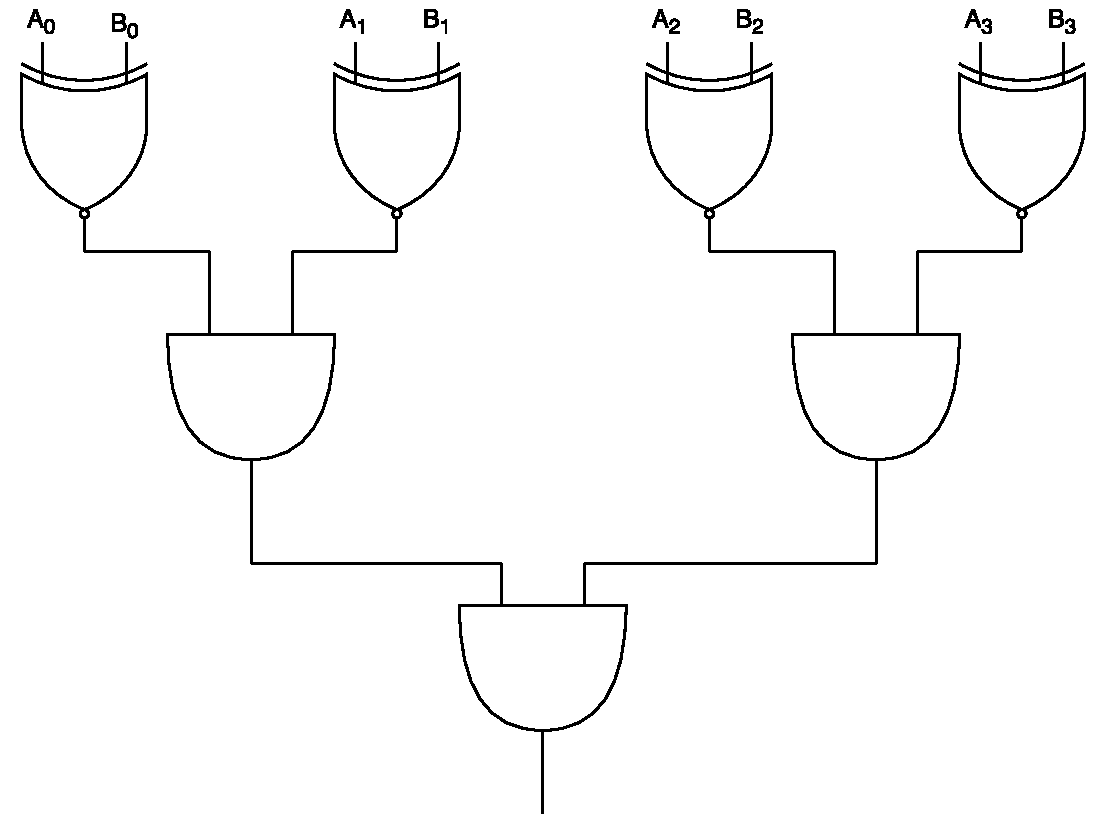
\includegraphics[width=\textwidth]{images/equal_circuit.pdf}
	\end{figure}

	\begin{figure}
		\caption{Garbled Circuit Wires}
		\label{fig:garbled_circuit}
		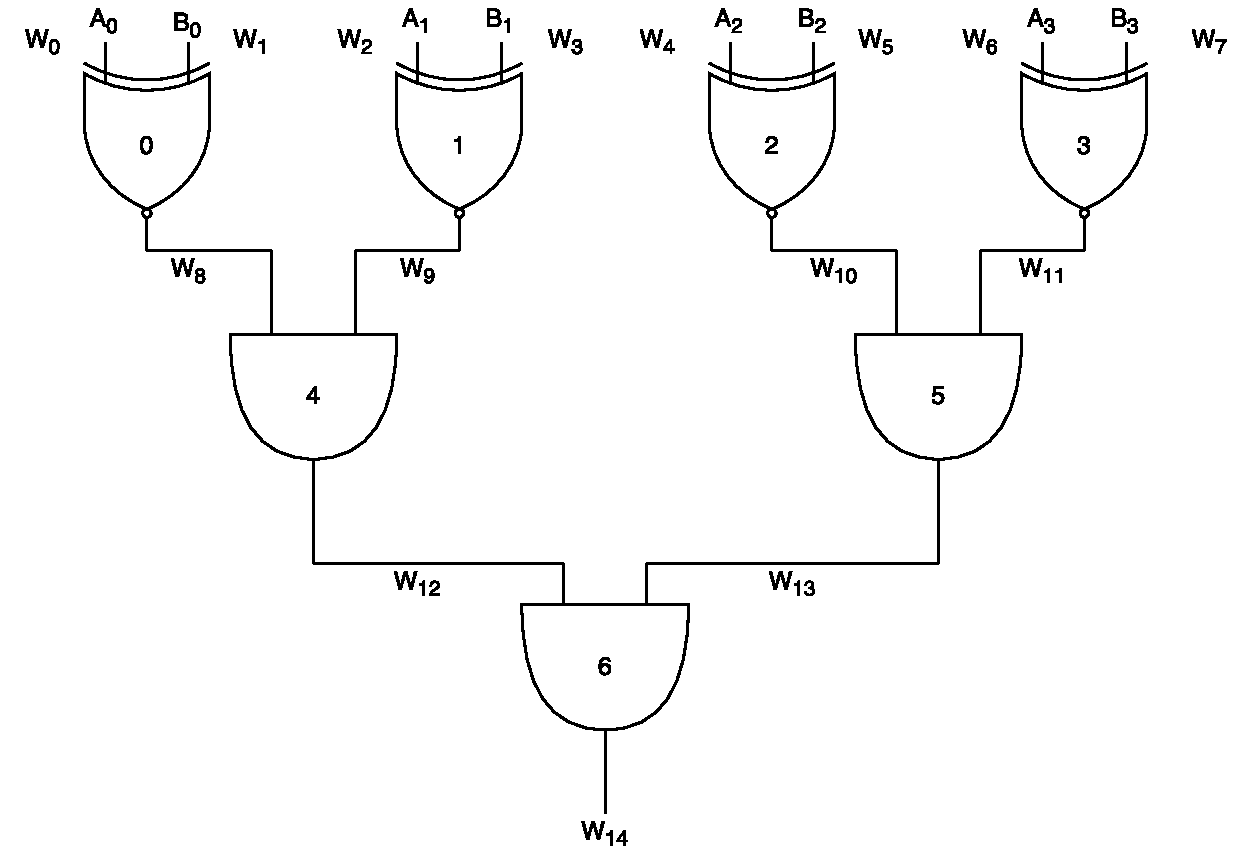
\includegraphics[width=\textwidth]{images/garbled_circuit.pdf}
	\end{figure}

	\begin{table}
		\centering
		\caption{Random t-bit Strings}
		\label{tab:random_string}
		\begin{tabular}{| c | c |}
			\hline
			$v_0^0$ = 00000000 & $v_0^1$ = 11111111 \\
			\hline
			$v_1^0$ = 00000001 & $v_1^1$ = 10000000 \\
			\hline
			$v_2^0$ = 00000010 & $v_2^1$ = 01000000 \\
			\hline
			$v_3^0$ = 00000011 & $v_3^1$ = 11000000 \\
			\hline
			$v_4^0$ = 00000100 & $v_4^1$ = 00100000 \\
			\hline
			$v_5^0$ = 00000101 & $v_5^1$ = 10100000 \\
			\hline
			$v_6^0$ = 00000110 & $v_6^1$ = 01100000 \\
			\hline
			$v_7^0$ = 00000111 & $v_7^1$ = 11100000 \\
			\hline
			$v_8^0$ = 00001000 & $v_8^1$ = 00010000 \\
			\hline
			$v_9^0$ = 00001001 & $v_9^1$ = 10010000 \\
			\hline
			$v_{10}^0$ = 00001010 & $v_{10}^1$ = 01010000 \\
			\hline
			$v_{11}^0$ = 00001011 & $v_{11}^1$ = 11010000 \\
			\hline
			$v_{12}^0$ = 00001100 & $v_{12}^1$ = 00110000 \\
			\hline
			$v_{13}^0$ = 00001101 & $v_{13}^1$ = 10110000 \\
			\hline
			$v_{14}^0$ = 00001110 & $v_{14}^1$ = 01110000 \\
			\hline
		\end{tabular}
	\end{table}

	\begin{table}
		\centering
		\caption{Permutation Bit}
		\label{tab:permutation}
		\begin{tabular}{| c |}
			\hline
			$p_{0}$ = 0 \\
			\hline
			$p_{1}$ = 1 \\
			\hline
			$p_{2}$ = 0 \\
			\hline
			$p_{3}$ = 1 \\
			\hline
			$p_{4}$ = 0 \\
			\hline
			$p_{5}$ = 1 \\
			\hline
			$p_{6}$ = 0 \\
			\hline
			$p_{7}$ = 1 \\
			\hline
			$p_{8}$ = 0 \\
			\hline
			$p_{9}$ = 1 \\
			\hline
			$p_{10}$ = 0 \\
			\hline
			$p_{11}$ = 1 \\
			\hline
			$p_{12}$ = 0 \\
			\hline
			$p_{13}$ = 1 \\
			\hline
			$p_{14}$ = 0 \\
			\hline
		\end{tabular}
	\end{table}

	\begin{table}
		\centering
		\caption{Wire Strings}
		\label{tab:wire}
		\begin{tabular}{| c | c |}
			\hline
			$w_0^0$ = 000000000 & $w_0^1$ = 111111111 \\
			\hline
			$w_1^0$ = 000000011 & $w_1^1$ = 100000000 \\
			\hline
			$w_2^0$ = 000000100 & $w_2^1$ = 010000001 \\
			\hline
			$w_3^0$ = 000000111 & $w_3^1$ = 110000000 \\
			\hline
			$w_4^0$ = 000001000 & $w_4^1$ = 001000001 \\
			\hline
			$w_5^0$ = 000001011 & $w_5^1$ = 101000000 \\
			\hline
			$w_6^0$ = 000001100 & $w_6^1$ = 011000001 \\
			\hline
			$w_7^0$ = 000001111 & $w_7^1$ = 111000000 \\
			\hline
			$w_8^0$ = 000010000 & $w_8^1$ = 000100001 \\
			\hline
			$w_9^0$ = 000010011 & $w_9^1$ = 100100000 \\
			\hline
			$w_{10}^0$ = 000010100 & $w_{10}^1$ = 010100001 \\
			\hline
			$w_{11}^0$ = 000010111 & $w_{11}^1$ = 110100000 \\
			\hline
			$w_{12}^0$ = 000011000 & $w_{12}^1$ = 001100001 \\
			\hline
			$w_{13}^0$ = 000011011 & $w_{13}^1$ = 101100000 \\
			\hline
			$w_{14}^0$ = 000011100 & $w_{14}^1$ = 011100001 \\
			\hline
		\end{tabular}
	\end{table}


	\begin{table}
		\centering
		\caption{GTT, EGTT, PEGTT for Gate 0}
		\label{tab:gtt0}
		\begin{adjustbox}{width=1\textwidth}
		\begin{tabular}{|c|c|c||c|c|c||c|c|c||c|c|c|}
			\hline
			\multicolumn{3}{|c||}{Truth Table} 		& 
				\multicolumn{3}{|c||}{GTT}			& 
					\multicolumn{3}{|c||}{EGTT} 		& 
						\multicolumn{3}{|c|}{PEGTT} \\
			\hline
			\hline
			X & Y & Out	& 
				X & Y & Out	& 
					X & Y & Out	& 
						X & Y & Out	\\
			\hline
			0 & 0 & 1 	&
				$w_{0}^0$	& $w_{1}^0$	& $w_{8}^1$	& 
					$Enc(w_{0}^0)$	& $Enc(w_{1}^0)$	& $Enc(w_{8}^1)$ &
						$Enc(w_{0}^1)$	& $Enc(w_{1}^0)$	& $Enc(w_{8}^0)$ \\
			\hline
			0 & 1 & 0 	&
				$w_{0}^0$	& $w_{1}^1$	& $w_{8}^0$	& 
					$Enc(w_{0}^0)$	& $Enc(w_{1}^1)$	& $Enc(w_{8}^0)$ &
						$Enc(w_{0}^1)$	& $Enc(w_{1}^1)$	& $Enc(w_{8}^1)$ \\
			\hline
			1 & 0 & 0 	&
				$w_{0}^1$	& $w_{1}^0$	& $w_{8}^0$	& 
					$Enc(w_{0}^1)$	& $Enc(w_{1}^0)$	& $Enc(w_{8}^0)$ &
						$Enc(w_{0}^0)$	& $Enc(w_{1}^0)$	& $Enc(w_{8}^1)$ \\
			\hline
			1 & 1 & 1 	&
				$w_{0}^1$	& $w_{1}^1$	& $w_{8}^1$	& 
					$Enc(w_{0}^1)$	& $Enc(w_{1}^1)$	& $Enc(w_{8}^1)$ &
						$Enc(w_{0}^0)$	& $Enc(w_{1}^1)$	& $Enc(w_{8}^0)$ \\
			\hline
		\end{tabular}
		\end{adjustbox}
	\end{table}

	\begin{table}
		\centering
		\caption{GTT, EGTT, PEGTT for Gate 1}
		\label{tab:gtt1}
		\begin{adjustbox}{width=1\textwidth}
		\begin{tabular}{|c|c|c||c|c|c||c|c|c||c|c|c|}
			\hline
			\multicolumn{3}{|c||}{Truth Table} 		& 
				\multicolumn{3}{|c||}{GTT}			& 
					\multicolumn{3}{|c||}{EGTT} 		& 
						\multicolumn{3}{|c|}{PEGTT} \\
			\hline
			\hline
			X & Y & Out	& 
				X & Y & Out	& 
					X & Y & Out	& 
						X & Y & Out	\\
			\hline
			0 & 0 & 1 	&
				$w_{2}^0$	& $w_{3}^0$	& $w_{9}^1$	& 
					$Enc(w_{2}^0)$	& $Enc(w_{3}^0)$	& $Enc(w_{9}^1)$ &
						$Enc(w_{2}^1)$	& $Enc(w_{3}^0)$	& $Enc(w_{9}^0)$ \\
			\hline
			0 & 1 & 0 	&
				$w_{2}^0$	& $w_{3}^1$	& $w_{9}^0$	& 
					$Enc(w_{2}^0)$	& $Enc(w_{3}^1)$	& $Enc(w_{9}^0)$ &
						$Enc(w_{2}^1)$	& $Enc(w_{3}^1)$	& $Enc(w_{9}^1)$ \\
			\hline
			1 & 0 & 0 	&
				$w_{2}^1$	& $w_{3}^0$	& $w_{9}^0$	& 
					$Enc(w_{2}^1)$	& $Enc(w_{3}^0)$	& $Enc(w_{9}^0)$ &
						$Enc(w_{2}^0)$	& $Enc(w_{3}^0)$	& $Enc(w_{9}^1)$ \\
			\hline
			1 & 1 & 1 	&
				$w_{2}^1$	& $w_{3}^1$	& $w_{9}^1$	& 
					$Enc(w_{2}^1)$	& $Enc(w_{3}^1)$	& $Enc(w_{9}^1)$ &
						$Enc(w_{2}^0)$	& $Enc(w_{3}^1)$	& $Enc(w_{9}^0)$ \\
			\hline
		\end{tabular}
		\end{adjustbox}
	\end{table}

	\begin{table}
		\centering
		\caption{GTT, EGTT, PEGTT for Gate 2}
		\label{tab:gtt2}
		\begin{adjustbox}{width=1\textwidth}
		\begin{tabular}{|c|c|c||c|c|c||c|c|c||c|c|c|}
			\hline
			\multicolumn{3}{|c||}{Truth Table} 		& 
				\multicolumn{3}{|c||}{GTT}			& 
					\multicolumn{3}{|c||}{EGTT} 		& 
						\multicolumn{3}{|c|}{PEGTT} \\
			\hline
			\hline
			X & Y & Out	& 
				X & Y & Out	& 
					X & Y & Out	& 
						X & Y & Out	\\
			\hline
			0 & 0 & 1 	&
				$w_{4}^0$	& $w_{5}^0$	& $w_{10}^1$	& 
					$Enc(w_{4}^0)$	& $Enc(w_{5}^0)$	& $Enc(w_{10}^1)$ &
						$Enc(w_{4}^1)$	& $Enc(w_{5}^0)$	& $Enc(w_{10}^0)$ \\
			\hline
			0 & 1 & 0 	&
				$w_{4}^0$	& $w_{5}^1$	& $w_{10}^0$	& 
					$Enc(w_{4}^0)$	& $Enc(w_{5}^1)$	& $Enc(w_{10}^0)$ &
						$Enc(w_{4}^1)$	& $Enc(w_{5}^1)$	& $Enc(w_{10}^1)$ \\
			\hline
			1 & 0 & 0 	&
				$w_{4}^1$	& $w_{5}^0$	& $w_{10}^0$	& 
					$Enc(w_{4}^1)$	& $Enc(w_{5}^0)$	& $Enc(w_{10}^0)$ &
						$Enc(w_{4}^0)$	& $Enc(w_{5}^0)$	& $Enc(w_{10}^1)$ \\
			\hline
			1 & 1 & 1 	&
				$w_{4}^1$	& $w_{5}^1$	& $w_{10}^1$	& 
					$Enc(w_{4}^1)$	& $Enc(w_{5}^1)$	& $Enc(w_{10}^1)$ &
						$Enc(w_{4}^0)$	& $Enc(w_{5}^1)$	& $Enc(w_{10}^0)$ \\
			\hline
		\end{tabular}
		\end{adjustbox}
	\end{table}

	\begin{table}
		\centering
		\caption{GTT, EGTT, PEGTT for Gate 3}
		\label{tab:gtt3}
		\begin{adjustbox}{width=1\textwidth}
		\begin{tabular}{|c|c|c||c|c|c||c|c|c||c|c|c|}
			\hline
			\multicolumn{3}{|c||}{Truth Table} 		& 
				\multicolumn{3}{|c||}{GTT}			& 
					\multicolumn{3}{|c||}{EGTT} 		& 
						\multicolumn{3}{|c|}{PEGTT} \\
			\hline
			\hline
			X & Y & Out	& 
				X & Y & Out	& 
					X & Y & Out	& 
						X & Y & Out	\\
			\hline
			0 & 0 & 1 	&
				$w_{6}^0$	& $w_{7}^0$	& $w_{11}^1$	& 
					$Enc(w_{6}^0)$	& $Enc(w_{7}^0)$	& $Enc(w_{11}^1)$ &
						$Enc(w_{6}^1)$	& $Enc(w_{7}^0)$	& $Enc(w_{11}^0)$ \\
			\hline
			0 & 1 & 0 	&
				$w_{6}^0$	& $w_{7}^1$	& $w_{11}^0$	& 
					$Enc(w_{6}^0)$	& $Enc(w_{7}^1)$	& $Enc(w_{11}^0)$ &
						$Enc(w_{6}^1)$	& $Enc(w_{7}^1)$	& $Enc(w_{11}^1)$ \\
			\hline
			1 & 0 & 0 	&
				$w_{6}^1$	& $w_{7}^0$	& $w_{11}^0$	& 
					$Enc(w_{6}^1)$	& $Enc(w_{7}^0)$	& $Enc(w_{11}^0)$ &
						$Enc(w_{6}^0)$	& $Enc(w_{7}^0)$	& $Enc(w_{11}^1)$ \\
			\hline
			1 & 1 & 1 	&
				$w_{6}^1$	& $w_{7}^1$	& $w_{11}^1$	& 
					$Enc(w_{6}^1)$	& $Enc(w_{7}^1)$	& $Enc(w_{11}^1)$ &
						$Enc(w_{6}^0)$	& $Enc(w_{7}^1)$	& $Enc(w_{11}^0)$ \\
			\hline
		\end{tabular}
		\end{adjustbox}
	\end{table}

	\begin{table}
		\centering
		\caption{GTT, EGTT, PEGTT for Gate 4}
		\label{tab:gtt4}
		\begin{adjustbox}{width=1\textwidth}
		\begin{tabular}{|c|c|c||c|c|c||c|c|c||c|c|c|}
			\hline
			\multicolumn{3}{|c||}{Truth Table} 		& 
				\multicolumn{3}{|c||}{GTT}			& 
					\multicolumn{3}{|c||}{EGTT} 		& 
						\multicolumn{3}{|c|}{PEGTT} \\
			\hline
			\hline
			X & Y & Out	& 
				X & Y & Out	& 
					X & Y & Out	& 
						X & Y & Out	\\
			\hline
			0 & 0 & 0 	&
				$w_{8}^0$	& $w_{9}^0$	& $w_{12}^0$	& 
					$Enc(w_{8}^0)$	& $Enc(w_{9}^0)$	& $Enc(w_{12}^0)$ &
						$Enc(w_{8}^1)$	& $Enc(w_{9}^0)$	& $Enc(w_{12}^0)$ \\
			\hline
			0 & 1 & 0 	&
				$w_{8}^0$	& $w_{9}^1$	& $w_{12}^0$	& 
					$Enc(w_{8}^0)$	& $Enc(w_{9}^1)$	& $Enc(w_{12}^0)$ &
						$Enc(w_{8}^1)$	& $Enc(w_{9}^1)$	& $Enc(w_{12}^1)$ \\
			\hline
			1 & 0 & 0 	&
				$w_{8}^1$	& $w_{9}^0$	& $w_{12}^0$	& 
					$Enc(w_{8}^1)$	& $Enc(w_{9}^0)$	& $Enc(w_{12}^0)$ &
						$Enc(w_{8}^0)$	& $Enc(w_{9}^0)$	& $Enc(w_{12}^0)$ \\
			\hline
			1 & 1 & 1 	&
				$w_{8}^1$	& $w_{9}^1$	& $w_{12}^1$	& 
					$Enc(w_{8}^1)$	& $Enc(w_{9}^1)$	& $Enc(w_{12}^1)$ &
						$Enc(w_{8}^0)$	& $Enc(w_{9}^1)$	& $Enc(w_{12}^0)$ \\
			\hline
		\end{tabular}
		\end{adjustbox}
	\end{table}

	\begin{table}
		\centering
		\caption{GTT, EGTT, PEGTT for Gate 5}
		\label{tab:gtt5}
		\begin{adjustbox}{width=1\textwidth}
		\begin{tabular}{|c|c|c||c|c|c||c|c|c||c|c|c|}
			\hline
			\multicolumn{3}{|c||}{Truth Table} 		& 
				\multicolumn{3}{|c||}{GTT}			& 
					\multicolumn{3}{|c||}{EGTT} 		& 
						\multicolumn{3}{|c|}{PEGTT} \\
			\hline
			\hline
			X & Y & Out	& 
				X & Y & Out	& 
					X & Y & Out	& 
						X & Y & Out	\\
			\hline
			0 & 0 & 0 	&
				$w_{10}^0$	& $w_{11}^0$	& $w_{13}^0$	& 
					$Enc(w_{10}^0)$	& $Enc(w_{11}^0)$	& $Enc(w_{13}^0)$ &
						$Enc(w_{10}^1)$	& $Enc(w_{11}^0)$	& $Enc(w_{13}^0)$ \\
			\hline
			0 & 1 & 0 	&
				$w_{10}^0$	& $w_{11}^1$	& $w_{13}^0$	& 
					$Enc(w_{10}^0)$	& $Enc(w_{11}^1)$	& $Enc(w_{13}^0)$ &
						$Enc(w_{10}^1)$	& $Enc(w_{11}^1)$	& $Enc(w_{13}^1)$ \\
			\hline
			1 & 0 & 0 	&
				$w_{10}^1$	& $w_{11}^0$	& $w_{13}^0$	& 
					$Enc(w_{10}^1)$	& $Enc(w_{11}^0)$	& $Enc(w_{13}^0)$ &
						$Enc(w_{10}^0)$	& $Enc(w_{11}^0)$	& $Enc(w_{13}^0)$ \\
			\hline
			1 & 1 & 1 	&
				$w_{10}^1$	& $w_{11}^1$	& $w_{13}^1$	& 
					$Enc(w_{10}^1)$	& $Enc(w_{11}^1)$	& $Enc(w_{13}^1)$ &
						$Enc(w_{10}^0)$	& $Enc(w_{11}^1)$	& $Enc(w_{13}^0)$ \\
			\hline
		\end{tabular}
		\end{adjustbox}
	\end{table}

	\begin{table}
		\centering
		\caption{GTT, EGTT, PEGTT for Gate 6}
		\label{tab:gtt6}
		\begin{adjustbox}{width=1\textwidth}
		\begin{tabular}{|c|c|c||c|c|c||c|c|c||c|c|c|}
			\hline
			\multicolumn{3}{|c||}{Truth Table} 		& 
				\multicolumn{3}{|c||}{GTT}			& 
					\multicolumn{3}{|c||}{EGTT} 		& 
						\multicolumn{3}{|c|}{PEGTT} \\
			\hline
			\hline
			X & Y & Out	& 
				X & Y & Out	& 
					X & Y & Out	& 
						X & Y & Out	\\
			\hline
			0 & 0 & 0 	&
				$w_{12}^0$	& $w_{13}^0$	& $w_{14}^0$	& 
					$Enc(w_{12}^0)$	& $Enc(w_{13}^0)$	& $Enc(w_{14}^0)$ &
						$Enc(w_{12}^1)$	& $Enc(w_{13}^0)$	& $Enc(w_{14}^0)$ \\
			\hline
			0 & 1 & 0 	&
				$w_{12}^0$	& $w_{13}^1$	& $w_{14}^0$	& 
					$Enc(w_{12}^0)$	& $Enc(w_{13}^1)$	& $Enc(w_{14}^0)$ &
						$Enc(w_{12}^1)$	& $Enc(w_{13}^1)$	& $Enc(w_{14}^1)$ \\
			\hline
			1 & 0 & 0 	&
				$w_{12}^1$	& $w_{13}^0$	& $w_{14}^0$	& 
					$Enc(w_{12}^1)$	& $Enc(w_{13}^0)$	& $Enc(w_{14}^0)$ &
						$Enc(w_{12}^0)$	& $Enc(w_{13}^0)$	& $Enc(w_{14}^0)$ \\
			\hline
			1 & 1 & 1 	&
				$w_{12}^1$	& $w_{13}^1$	& $w_{14}^1$	& 
					$Enc(w_{12}^1)$	& $Enc(w_{13}^1)$	& $Enc(w_{14}^1)$ &
						$Enc(w_{12}^0)$	& $Enc(w_{13}^1)$	& $Enc(w_{14}^0)$ \\
			\hline
		\end{tabular}
		\end{adjustbox}
	\end{table}
	
	
		
\end{document}